\documentclass{article}
\usepackage{fancyhdr}
\usepackage{amsthm}
\usepackage{etoolbox}
\usepackage{verbatim}
\usepackage{enumerate}
\usepackage{amsmath}
\usepackage{algorithmicx}
\usepackage{algorithm}
\usepackage{algpseudocode}
\usepackage{amssymb}
\usepackage{tikz}
	
\pagestyle{fancy}
\title{Chapter 32}
\author{Michelle Bodnar, Andrew Lohr}

\newcounter{curnum}
\setcounter{curnum}{0}

\newtheorem{th1}{Exercise} 
\newcommand{\calH}{\mathcal{H}}
\newcommand{\calX}{\mathcal{X}}
\newcommand{\calA}{\mathcal{A}}
\newcommand{\calY}{\mathcal{Y}}
\newcommand{\Z}{\mathbb{Z}}



\algblock{ParFor}{EndParFor}
% customising the new block
\algnewcommand\algorithmicparfor{\textbf{parallel for}}
\algnewcommand\algorithmicpardo{\textbf{do}}
\algnewcommand\algorithmicendparfor{\textbf{end}}
\algrenewtext{ParFor}[1]{\algorithmicparfor\ #1\ \algorithmicpardo}
\algrenewtext{EndParFor}{\algorithmicendparfor}

\begin{document}
\maketitle
\noindent\textbf{Exercise 32.1-1}\\

We let $(i,j)$ denote that the algorithm checks index $i$ of the text against index $j$ of the pattern. We'll let p(s) indicate that the matching algorithm reported an occurrence with a shift of $s$. The algorithm has the following execution on $T = 000010001010001$ and $P = 0001$.

\[
\begin{array}{|c|ccccc|}
\hline
s=0&(0,0)&(1,1)&(2,2)&(3,3)&\\
s=1&(1,0)&(2,1)&(3,2)&(4,3)&p(1)\\
s=2&(2,0)&(3,1)&(4,2)&&\\
s=3&(3,0)&(4,1)&&&\\
s=4&(4,0)&&&&\\
s=5&(5,0)&(6,1)&(7,2)&(8,3)&p(5)\\
s=6&(6,0)&(7,1)&(8,2)&&\\
s=7&(7,0)&(8,1)&&&\\
s=8&(8,0)&&&&\\
s=9&(9,0)&(10,1)&&&\\
s=10&(10,0)&&&&\\
s=11&(11,0)&(12,1)&(13,2)&(14,3)&p(11)\\
\hline
\end{array}
\]

\noindent\textbf{Exercise 32.1-2}\\

We know that one occurrence of $P$ in $T$ cannot overlap with another, so we don't need to double-check the way the naive algorithm does.  If we find an occurrence of $P_k$ in the text followed by a nonmatch, we can increment $s$ by $k$ instead of 1.  It can be modified in the following way:\\

\begin{algorithm}
\caption{DISTINCT-NAIVE-STRING-MATCHER$(T,P)$}
\begin{algorithmic}
\State $n = T.length$ 
\State $m = P.length$
\State $k=0$
\While{$s \leq n-m$}
	\State $i=1$
	\If{$T[s] == P[1]$}
		\State $k = s$
		\State $i=0$
		\While{$T[k+i] == P[i]$ and $i < m$}
			$i = i+1$
			\If{$i == m$}
				\State Print ``Pattern occurs with shift'' $k$
			\EndIf
		\EndWhile
	\EndIf
	\State $s = s+i$
\EndWhile
\end{algorithmic}
\end{algorithm}

\noindent\textbf{Exercise 32.1-3}\\

For any particular value of $s$, the probability that the $i$th character will need to be looked at when doing the string comparison is the probability that the first $i-1$ characters matched, which is $\frac{1}{d^{i-1}}$. So, by linearity of expectation, summing up over all $s$ and $i$, we have that the expected number of steps is, by equation (A.5),

\begin{align*}
(n-m+1) \sum_{i=1}^{m} \frac{1}{d^{i-1}}&=  (n-m+1)\left(\frac{(d^{-m}-1)}{(d^{-1}-1)}\right)\\
&= (n-m+1)(\frac{1-d^{-m}}{1-d^{-1}}) \\
&\le (n-m+1) \frac{1}{1-d^{-1}}\\
&\le (n-m+1) \frac{1}{1-\frac{1}{2}}\\
& = 2(n-m+1)
\end{align*}


\noindent\textbf{Exercise 32.1-4}\\

We can decompose a pattern with $g-1$ gap characters into the form $a_1 \diamond a_2 \diamond \cdots \diamond a_g$.  Since we only care whether or not the pattern appears somewhere, it will suffice to look for the first occurrence of $a_1$, followed by the first occurrence of $a_2$ which comes anywhere after $a_1$, and so on.  If the pattern $P$ has length $m$ and the text has length $n$ then the runtime of the naive strategy is $O(nm)$.\\

\noindent\textbf{Exercise 32.2-1}\\

Since the string $26$ only appears once in the text, to find the number of spurious hits, we will find the total number of hits and subtract 1. when we compute the hash of the pattern we get $(20 + 6)\mod 11 \equiv 26\mod 11 \equiv 4\mod 11$.

We get the following hashes of various shift values:

\[
\begin{array}{|cc|}
\hline 
s&t_s\\
\hline
0&9\\
1&3\\
2&8\\
3&4\\
4&4\\
5&4\\
6&4\\
7&10\\
8&9\\
9&2\\
10&3\\
11&1\\
12&9\\
13&2\\
14&5\\
\hline
\end{array}
\]

Since there were 4 hits, three of them must of been spurious.\\

\noindent\textbf{Exercise 32.2-2}\\

We first tackle the case where each of the $k$ patterns has the same length $m$.  We first compute the number associated to each pattern in $O(m)$ time, which contributes $O(km)$ to the runtime.  In line 10 we make $k$ checks, one for each pattern, which contributes $O(n-m+1)km$ time.  Thus, the total runtime is $O(km(n-m+1)$. For patterns of different lengths $l_1, l_2, \ldots, l_k$, keep an array $A$ such that $A[i]$ holds the number associated to the first $l_i$ digits of $T$, mod $q$.  We'll have to update each of these each time the outer for-loop is executed, but it will allow us to immediately compare any of the pattern numbers to the appropriate text number, as done in line 10. \\

\noindent\textbf{Exercise 32.2-3}\\

We use the same idea of maintaining a hash of the pattern and computing running hashes of the text. However, updating the hash at each step can take time as long as $\Theta(m)$ because the number of entries which are both entering and leaving the hashed window is $2m$, and you have to at least look at all of them as they come in and leave. This would get us a total expected runtime (occurring not too many spurious hits of $(n-m+1)^2\cdot m$, and still the same worst case as the trivial algorithm, which is $(n-m+1)^2 \cdot m^2$.

In order to compute this hash, we will be giving each entry of the window a power of $d$ that unique to its position. The entry in row $i$, column $j$ will be multiplied by $d^{m^2 - mi + j}$. Then, moving to the right, we multiply the value of the hash by $d$, subtract off the scaled entries that were in the left column, and add in the entries that are in the right column, also appropriately scaled by what row they are in. Similarly for shifting the window up or down. Again, all of this arithmetic is done mod some large prime.\\

\noindent\textbf{Exercise 32.2-4}\\

Suppose $A(x) = B(x)$.  Then $\sum_{i=0}^{n-1}(a_i-b_i)x^i \equiv 0 \mod q$.  Since $q$ is prime, Exercise 31.4-4 tells us that this equation has at most $n-1$ solutions modulo $q$. Since each of the $q$ choices for $x$ is equally likely, the probability that we pick one of the potential $n-1$ which make the equation hold is $(n-1)/q < (n-1)/1000n < 1/1000$. However, if the files are the same then $a_i = b_i$ for all $i$, so $A(x) = B(x)$. \\


\noindent\textbf{Exercise 32.3-1}\\

The states will be $\{0,1,2,3,4,5,6\}$ and having a transition function given by

\[
\begin{array}{|c|cc|}
\hline
\hbox{state}&a&b\\
\hline
0&1&0\\
1&2&0\\
2&2&3\\
3&4&0\\
4&2&5\\
5&1&0\\
\hline
\end{array}
\]

The sequence of states for $T$ is $0,1,2,2,3,4,5,1,2,3,4,2,3,4,5,1,2,3$, and so finds two occurrences of the pattern, one at $s=1$ and another at $s= 9$.

\noindent\textbf{Exercise 32.3-2}\\

See picture below for the 22 state automaton.\\

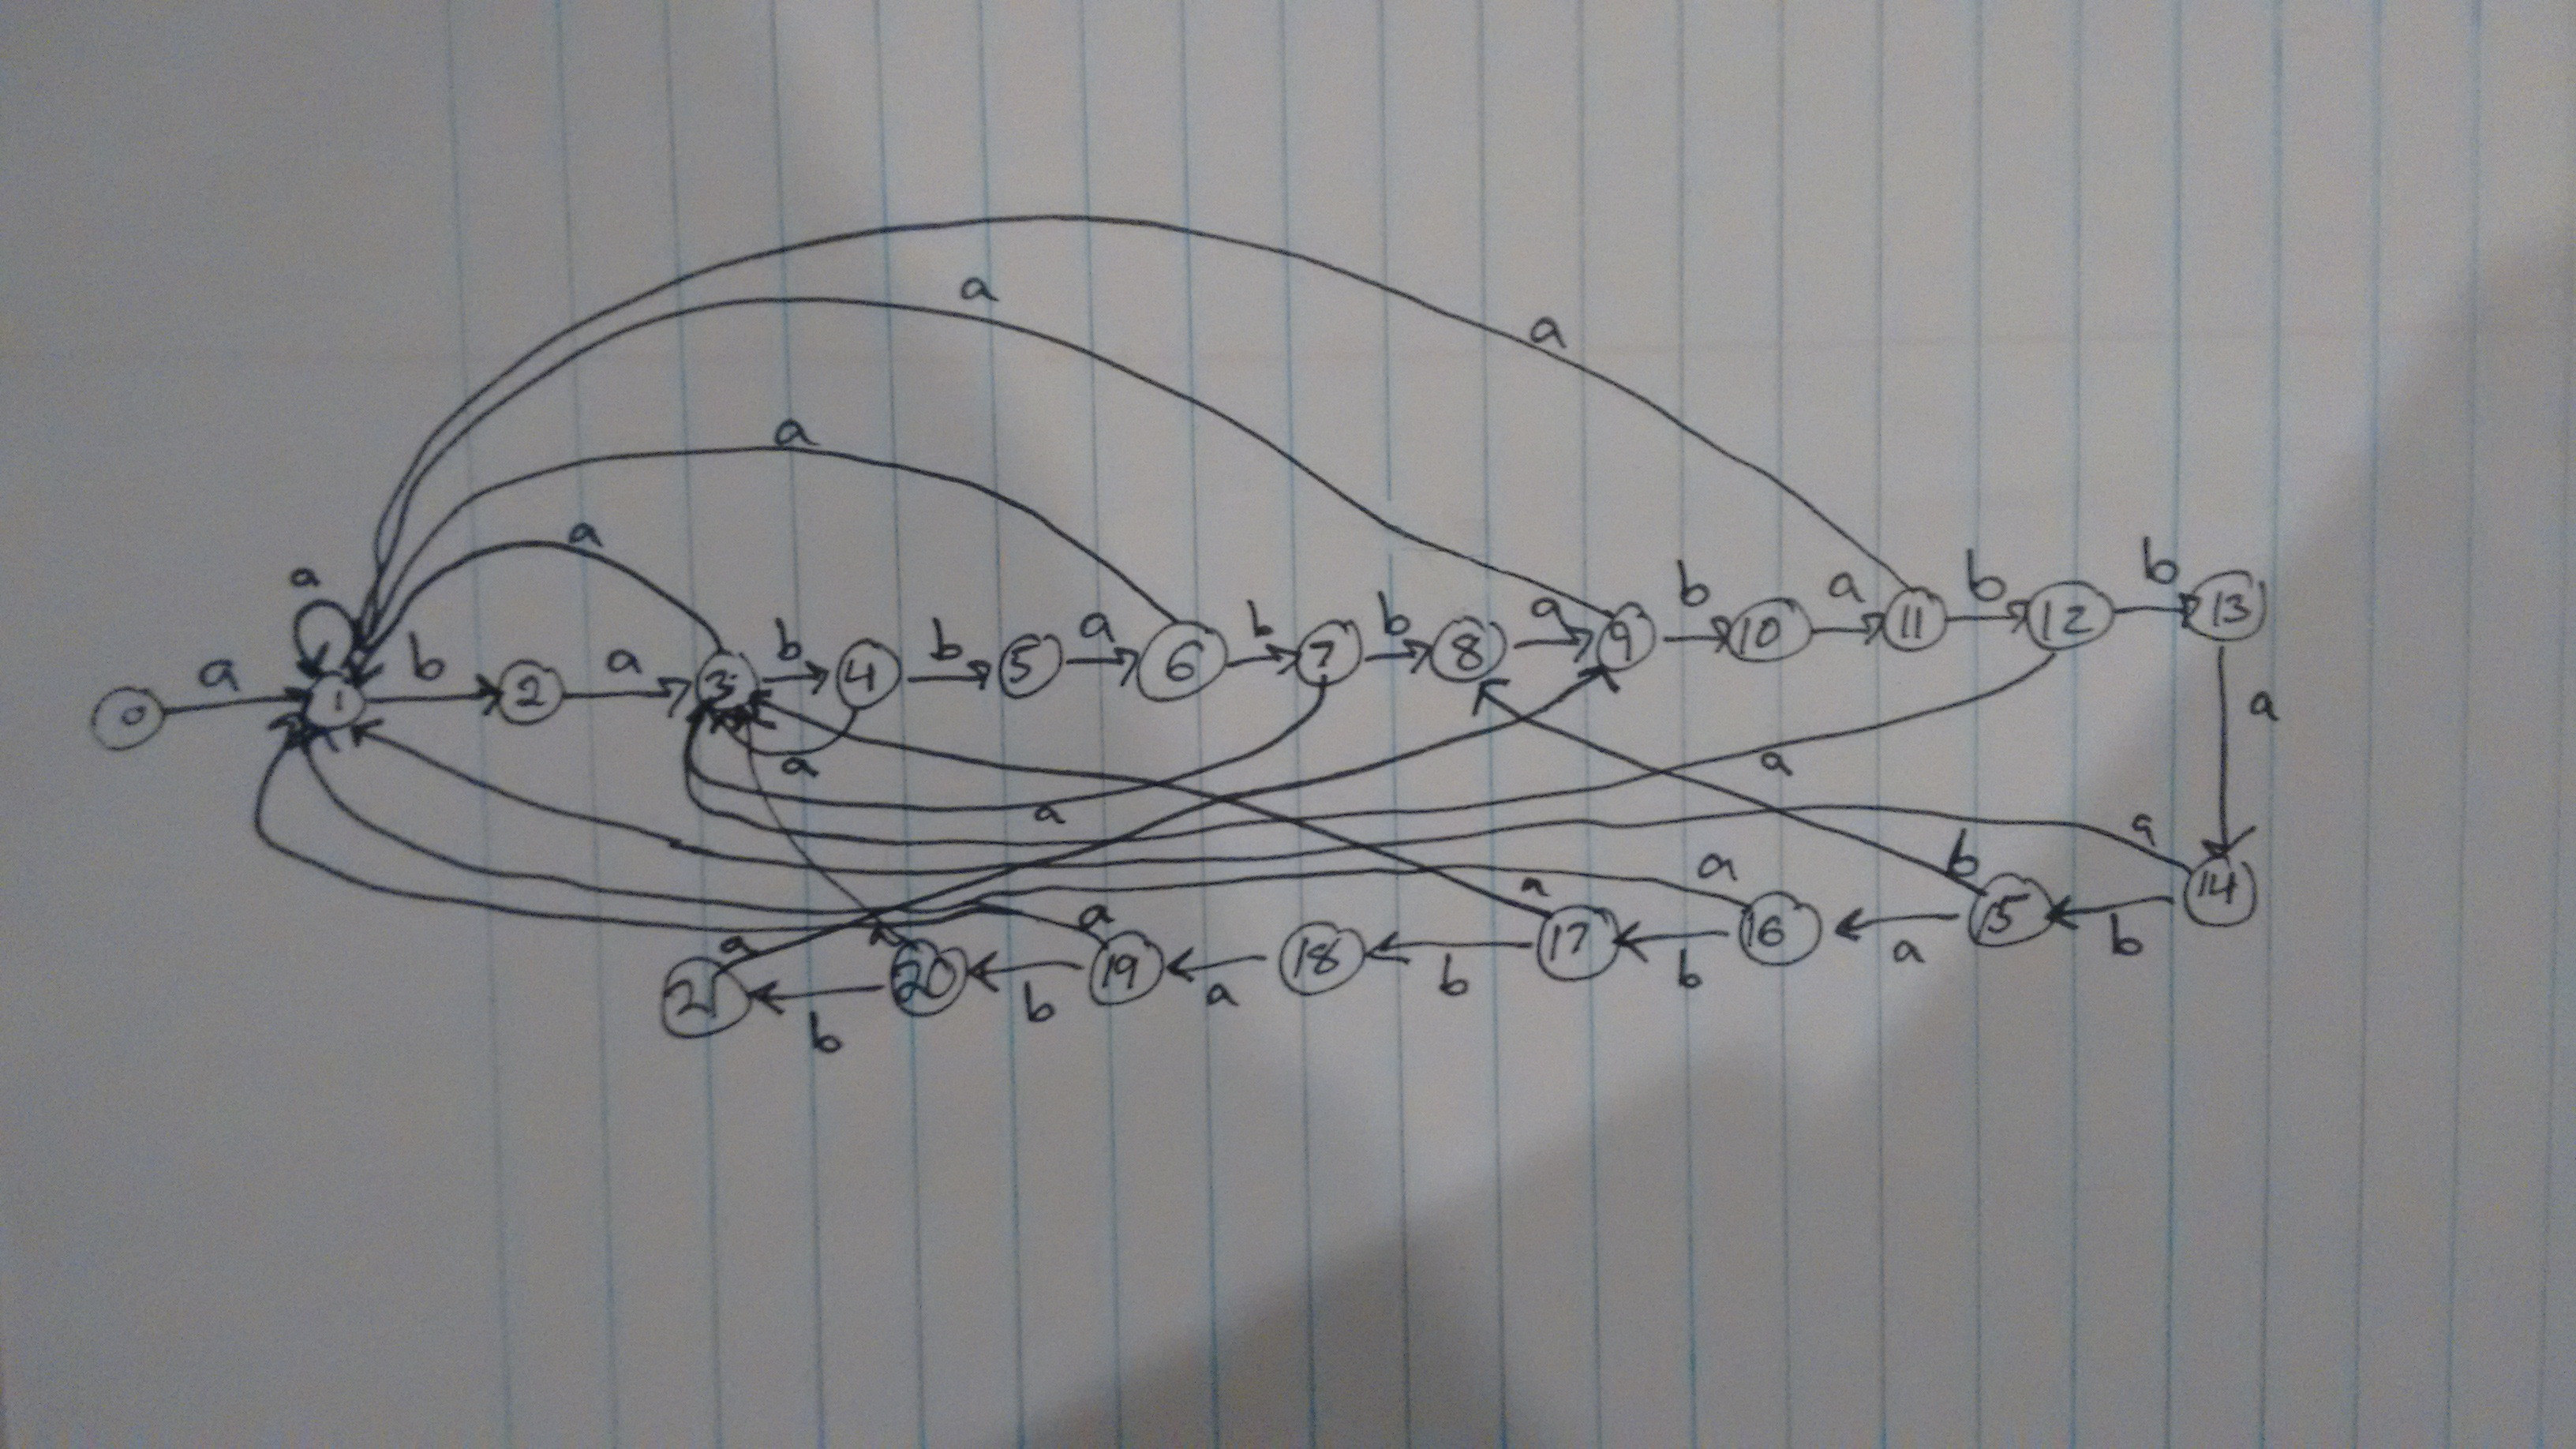
\includegraphics[scale=.1]{automaton.jpg}\\

\noindent\textbf{Exercise 32.3-3}\\

The state transition function looks like a straight line, with all other edges going back to either the initial vertex (if it is not the first letter of the patter) or the second vertex (if it is the first letter of the pattern). If it were to go back to any later state, that would mean that some suffix of what we had constructed so far(which was a prefix of P) was a prefix of the copy of $P$ that we are next trying to find.\\


\noindent\textbf{Exercise 32.3-4}\\

We can construct the automaton as follows: Let $P_k$ be the longest prefix which both $P$ and $P'$ have in common.  Create the automaton $F$ for $P_k$ as usual. Add an arrow labeled $P[k+1]$ from state $k$ to a chain of states $k+1, k+2, \ldots, |P|$, and draw the appropriate arrows, so that $\delta(q,a) = \sigma(P_q a)$.  Next, add an arrow labeled $P'[k+1]$ from state $k$ to a chain of states $(k+1)', (k+2)', \ldots, |P'|'$. Draw the appropriate arrows so that $\delta(q,a) = \sigma(P'_qa)$. \\

\noindent\textbf{Exercise 32.3-5}\\

To create a DFA that worked with gap characters, construct the DFA so that it has $|P|+1$ states. let $m$ be the number of gap characters Suppose that the positions of all the gap characters within the pattern $p$ are given by $g_i$, and let $g_0=0$, $g_m = |P|+1$. Let the segment of pattern occurring after gap character $i$ but before the $i+1$ gap character be called $P_i$. Then, we will imagine that we are trying to match each of these patterns in sequence, but if we have trouble matching some particular pattern, then we can not undo the success we enjoyed in matching earlier patterns. 

More concretely, suppose that we have $(Q_i,q_{i,0},A_i,\Sigma_i,\delta_i)$ is the DFA corresponding to the pattern $P_i$. Then, we will construct our DFA so that $Q = \sqcup_i Q_i$, $q_0 = q_{0,0}$, $A = A_{m+1}$, $\Sigma = \cup_i \Sigma_i$, and $\delta$ is described below. If we are at state $q\in Q_i$ and see character $a$, if $q\not\in A_i$, we just go to the state proscribed by $\delta_i(q,a)$. If, however, we have that $q \in A_i$, then, $\delta(q,a) = \delta_{i+1}(q_{i+1,0},a)$. This construction achieves the description given in English above.\\


\noindent\textbf{Exercise 32.4-1}\\

The prefix function is:

\[
\begin{array}{|cc|}
\hline
i &\pi(i)\\
\hline
1&0\\
2&0\\
3&1\\
4&2\\
5&0\\
6&1\\
7&2\\
8&0\\
9&1\\
10&2\\
11&0\\
12&1\\
13&2\\
14&3\\
15&4\\
16&5\\
17&6\\
18&7\\
19&8\\
\hline
\end{array}
\]

\noindent\textbf{Exercise 32.4-2}\\

The largest $\pi^*[q]$ can be is $q-1$.  This is tight because if $P$ consists of a the letter $a$ repeated $m$ times, the $\pi^*[q] = q-1$ for all $q$. \\



\noindent\textbf{Exercise 32.4-3}\\

Suppose that at position $i$, you have the value of the prefix function is $\pi[i]$. Then, if $i-\pi[i] \ge|P| $, this means that there is an occurrence of $|P|$ starting at position $i-\pi[i]$. 

A simpler way to achieve a similar result is to expand the alphabet by one, making it so that some character $c$ does not occur in either $P$ or $T$, then compute the prefix array of $PcT$, then, the prefix function is bounded by $|P|$ and any time that it reaches that bound, we have that there is an occurrence of the pattern, since we know that any prefix containing the $c$ cannot be a proper suffix of any other prefix.\\

\noindent\textbf{Exercise 32.4-4}\\

To show that the running time of KMP-MATCHER is $O(n)$, we'll show that the total number of executions of the while loop of line 6 is $O(n)$.  Observe that for each iteration for the for loop of line 5, $q$ increases by at most 1, in line 9.  This is because $\pi(q) < q$.  On the other hand, the while loop decreases $q$.  Since $q$ can never be negative, we must decrease $q$ fewer than $n$ times in total, so the while loop executes at most $n-1$ times.  Thus, the total runtime is $O(n)$. \\


\noindent\textbf{Exercise 32.4-5}\\

Basically, each time that we have to execute line 7, we have that we are decreasing $q$ by at least 1. Since the only place that we ever increase the value of $q$ is on line 9, and then we are only increasing it by 1, each of these runs of line 5 are paid for by the times we ran 9.

Using this as our motivation, we let the potential function be proportional to the value of $q$. This means that when we execute line 9, we pay a constant amount to raise up the potential function. And when we run line 7, we decrease the potential function which reduces the ammortized cost of an iteration of the while loop on line 6 to a zero amortized cost. The only other time that we change the value of q is on line 12, which only gets run once per execution of the outer for loop anyways and the amortization is in our favor there.

Since the ammortized cost under this potential function of each iteration of the outermost for loop is constant, and that loop runs $n$ times, the total cost of the algorithm is $\Theta(n)$.\\

\noindent\textbf{Exercise 32.4-6}\\

We'll prove this by induction on the number of recursive calls to $\pi'$.  The behavior is identical to $\pi$ if we are in the first or third cases (base cases) of the definition of $\pi'$, so the behavior is correct for a single call. Otherwise, $\pi'[q] = \pi'[\pi[q]]$.  The conditions of case 2 imply that the while loop of line 6 will execute an additional time after the update of line 7, so it is equivalent to setting $q = \pi[\pi[q]]$, and then continuing with the while loop as usual.  Since $\pi'$ recurses on $\pi[q]$ one fewer times than on $q$, its behavior is correct on $\pi[q]$, proving that the modified algorithm is correct.   KMP-MATCHER already runs asymptotically as fast as possible, so this doesn't constitute a runtime improvement in the worst case.  However, every time a recursive call to $\pi'$ is made, we circumvent having to check $P[q+1]$ against $T[i]$.\\

\noindent\textbf{Exercise 32.4-7}\\

If the lengths to $T$ and $T'$ are different, they are obviously not cyclic rotations of each other, so suppose that $|T|=T'$. Let our text be $TT$ and our pattern be $T'$. If and only if $T'$ occurs in $TT$, then the two given strings are cyclic rotations of each other. This can be done in linear time by the Knuth Morris Pratt algorithm.

To see that being cyclic rotations means that $T'$ occurs in $TT$, suppose that $T'$ is obtained from $T$ by cyclically shifting the right character to the left $s$ times. This means that the $|T|-s$ prefix of $T$ is a suffix of $T'$, and the $s$ suffix of $T$ is a prefix of $T'$. This means that $T'$ occurs in $TT$ with a shift of $|T|-s$.

Now, suppose that $T'$ occurs in $TT$ with a shift of $s$. This means that the $s$ suffix of $T$ is a prefix of $T'$, it also means that the $|T|-s$ characters left over in $T'$ are a prefix of $T$. So, they are cyclic rotations of each other.\\

\noindent\textbf{Exercise 32.4-8}\\

We have $\delta(q,a) = \sigma(P_qa)$, which is the length of the longest prefix of $P$ which is a suffix of $P_q a$.  Let this be $k$.  Then $P[1] = P[q-k+2]$, $P[2] = P[q-k+3], \ldots, P[k-1] = P[q], P[k] = a$.  On the other hand, $\delta(\pi[q],a) = \sigma(P_{\pi[q]}a)$.  It is clear that $\sigma(P_q a) \geq \sigma(P_{\pi[q]}a)$.  However, $\pi[q] \geq k-1$ and since $P[k] = a$, we must have $\sigma(P_{\pi[q]}a) \geq k$.  Thus, they are equal.   If $q \neq m$ and $P[q+1] = a$ then $\delta(q,a) = q+1$.  We can now compute the transition function $\delta$ in $O(m|\Sigma|)$ in the algorithm TRANSITION-FUNCTION, given below. \\

\begin{algorithm}
\caption{TRANSITION-FUNCTION$(P,\Sigma)$}
\begin{algorithmic}
\State $\pi = $ COMPUTE-PREFIX-FUNCTION$(P)$
\For{$a \in \Sigma$}
	\State $\delta(0,a) = 0$
\EndFor
\State $\delta(0,P[1]) = 1$
\For{$a \in \Sigma$}
	\For{$q=1$ to $m$}
		\If{$q == m$ or $P[q+1] \neq a$}
			\State $\delta(q,a) = \delta(\pi[q],a)$
		\Else
			\State $\delta(q,a) = q+1$
		\EndIf
	\EndFor
\EndFor
\end{algorithmic}
\end{algorithm}


\noindent\textbf{Problem 32-1}\\
\begin{enumerate}[a.]
\item
First, compute the prefix array for the given pattern in linear time using the method of section 32.4. Then, Suppose that $\pi[i] = i-k$. If $k | i$, we know that $k$ is the length of the primitive root, so, the word has a repetition factor of $\frac{i}{k}$. We also know that there is no smaller repetition factor in this case because otherwise we could include one more power of that root.

Now, suppose that we have $k$ not dividing $i$. We will show that we can only have the trivial repetition factor of $1$. Suppose we had some repetition $y^r = P_i$. Then, we know that $\pi[i] \ge y^{r-1}$. however, if we have it strictly greater than this, this means that we can write the y's themselves as powers because we have them aligning with themselves.

Since the only difficult step of this was finding the prefix function, which takes linear time, the runtime of this procedure is linear.
\item
To determine the probability that there is a repetition factor of $r$, we assign whatever we want to the first $\frac{i}{r}$ letters, and after that, all of the other letters are determined. This means that position $i$ has a repetition factor of $r$ with probability $\frac{1}{2^{i\frac{(r-1)}{r}}}$ for every $r$ dividing $i$. By applying a union bound to this, we have that the probability that $P_i$ has a repetition factor of more than $r$ is bounded by

\begin{align*}
\sum_{r'>r, r'|i} \frac{1}{2^{i\frac{(r'-1)}{r'}}}& = \frac{1}{2^i}\sum_{r'>r, r' |i}2^{i/r'}\\
&= \frac{1}{2^i} \sum_{j=1}^{\lfloor\frac{i/r}\rfloor}2^{j}\\
&\le \frac{2^{i/r}}{2^{i-1}}\\
&=2^{i/r -i +1}
\end{align*}

Then, applying the union bound over all values of $i$, we have the probability that a repetition factor of at least $r$ is bounded by

\begin{align*}
\sum_{i=0}^m 2^{i/r -i +1}& = 2 \sum_{i=1}^m 2^{(\frac{1}{r}-1)^i } \\
&= 2\frac{1-2^{\frac{m+1}{r}-m-1}}{1 - 2^{(\frac{1}{r}-1)}}\\
&\le 2\frac{1}{2^{(\frac{1}{r}-1)}}
\end{align*}

This shrinks quickly enough in $r$, that the expected value is finite, and since there is no $m$ in the expression, we have the expected value is bounded by a constant.
\item
This algorithm correctly finds the occurrences of the pattern $P$ for reasons similar to the Knuth Morris Pratt algorithm. That is, we know that we will only increase $q$ $\rho^*(P)$ many times before we have to bite the bullet and increase $s$, and $s$ can only be increased at most $n-m$ many times. It will definitely find every possible occurrence of the pattern because it searches for every time that the primitive root of $P$ occurs, and it must occur for $P$ to occur.
\end{enumerate}

\end{document}